% ============================================================
%  يُترجَم بـ XeLaTeX  (في Overleaf: Menu → Compiler → XeLaTeX)
%  الخط: Amiri (متوفر في Overleaf، أو حمّله من github.com/aliftype/amiri)
% ============================================================
\documentclass[12pt,a4paper]{article}
\usepackage[a4paper,margin=1.7cm,top=2.3cm,bottom=2.9cm,headheight=15pt,footskip=1.5cm]{geometry}
\usepackage{amsmath,amssymb}
\usepackage{icomma}
\usepackage[english,bidi=default,layout=lists]{babel}
\babelprovide[import,main]{arabic}
\babelfont{rm}[Scale=1.08]{Amiri}
\babelfont{sf}[Scale=1.08]{Amiri}
\usepackage[most]{tcolorbox}
\usepackage{tikz}
\usetikzlibrary{arrows.meta,calc,shadings}
\usepackage{array}
\usepackage{colortbl}
\usepackage{fancyhdr}
\usepackage{titlesec}
\usepackage{enumitem}
\usepackage{collcell}
\usepackage{needspace}
\usepackage{etoolbox}
% أعمدة جداول تُكتب خلاياها بالعربية في الاتجاه الصحيح
\newcolumntype{C}{>{\collectcell\ar}c<{\endcollectcell}}
% تجنب عنوان يتيم في أسفل الصفحة
\pretocmd{\section}{\Needspace{15\baselineskip}}{}{}
\pretocmd{\subsection}{\Needspace{11\baselineskip}}{}{}

% ---------- الألوان ----------
\definecolor{cDef}{HTML}{1F4E9C}
\definecolor{cThm}{HTML}{B3261E}
\definecolor{cRem}{HTML}{2E7D32}
\definecolor{cEx}{HTML}{C76B00}
\definecolor{cMeth}{HTML}{6A1B9A}
\definecolor{cSol}{HTML}{00695C}
\definecolor{cSec}{HTML}{1F3A68}

% ---------- العناوين ----------
\titleformat{\section}{\Large\bfseries\color{cSec}}{\thesection.}{0.6em}{}[{\color{cSec!60}\titlerule[1pt]}]
\titleformat{\subsection}{\large\bfseries\color{cThm!85!black}}{\thesubsection.}{0.5em}{}
\titlespacing*{\section}{0pt}{14pt}{8pt}
\titlespacing*{\subsection}{0pt}{10pt}{5pt}
\setlength{\parindent}{0pt}
\setlength{\parskip}{4pt}
\setlist{itemsep=2pt,topsep=3pt}

% ---------- الصناديق (تُرسم في سياق LTR ويُكتب محتواها بالعربية) ----------
\newtcolorbox{arbox}[3][]{enhanced,
  colback=#2!5,colframe=#2!80!black,arc=2mm,boxrule=0.8pt,
  left=6pt,right=6pt,top=8pt,bottom=5pt,
  fonttitle=\bfseries,coltitle=white,
  title={\foreignlanguage{arabic}{#3}},
  attach boxed title to top right={xshift=-5mm,yshift=-3mm},
  boxed title style={colback=#2!80!black,arc=1.5mm,boxrule=0pt},
  before upper={\selectlanguage{arabic}},
  before skip=8pt,after skip=8pt,breakable,#1}
\newenvironment{BOX}[2]{\begin{otherlanguage}{english}\begin{arbox}{#1}{#2}}{\end{arbox}\end{otherlanguage}}
\newenvironment{tarif}[1][تعريف]{\begin{BOX}{cDef}{#1}}{\end{BOX}}
\newenvironment{khassia}[1][خاصية]{\begin{BOX}{cThm}{#1}}{\end{BOX}}
\newenvironment{molahada}[1][ملاحظة]{\begin{BOX}{cRem}{#1}}{\end{BOX}}
\newenvironment{mithal}[1][مثال]{\begin{BOX}{cEx}{#1}}{\end{BOX}}
\newenvironment{tariqa}[1][طريقة]{\begin{BOX}{cMeth}{#1}}{\end{BOX}}

% ---------- التمارين والحلول ----------
\newcounter{exo}
\newenvironment{tamrin}[1]{\stepcounter{exo}\begin{BOX}{cSec}{التمرين \theexo: #1}}{\end{BOX}}
\newenvironment{hal}{\Needspace{12\baselineskip}\begin{otherlanguage}{english}\begin{arbox}[breakable]{cSol}{حل التمرين \theexo}}{\end{arbox}\end{otherlanguage}}

% رسومات TikZ تُوضع في سياق LTR
\newenvironment{LTR}{\begin{otherlanguage}{english}}{\end{otherlanguage}}
\newcommand{\ar}[1]{\foreignlanguage{arabic}{#1}}

% ---------- رموز ----------
% نقاط الحذف داخل الرياضيات (\dots يسبب خللاً في الاتجاه مع babel)
\renewcommand{\dots}{\mathinner{\ldotp\ldotp\ldotp}}
\renewcommand{\ldots}{\mathinner{\ldotp\ldotp\ldotp}}
\renewcommand{\cdots}{\mathinner{\cdotp\cdotp\cdotp}}
\newcommand{\N}{\mathbb{N}}
\newcommand{\Z}{\mathbb{Z}}
\newcommand{\D}{\mathbb{D}}
\newcommand{\Q}{\mathbb{Q}}
\newcommand{\R}{\mathbb{R}}
\newcommand{\pgcd}{\operatorname{PGCD}}
\newcommand{\ppcm}{\operatorname{PPCM}}

% ---------- تمثيل مجال على مستقيم عددي ----------
% \NLseg{a}{b}{[}{]}  مجال محدود
\newcommand{\NLseg}[4]{\begin{LTR}\begin{tikzpicture}[baseline=-0.6ex]
 \draw[-{Stealth[length=2mm]},gray!70](0,0)--(3.4,0);
 \draw[line width=2pt,cThm!80!black](0.7,0)--(2.7,0);
 \node[cThm!80!black,font=\LARGE] at (0.7,0){$#3$};
 \node[cThm!80!black,font=\LARGE] at (2.7,0){$#4$};
 \node[below=3pt,font=\footnotesize] at (0.7,0){$#1$};
 \node[below=3pt,font=\footnotesize] at (2.7,0){$#2$};
\end{tikzpicture}\end{LTR}}
% \NLright{a}{[}  مجال نحو +∞
\newcommand{\NLright}[2]{\begin{LTR}\begin{tikzpicture}[baseline=-0.6ex]
 \draw[-{Stealth[length=2mm]},gray!70](0,0)--(3.4,0);
 \draw[line width=2pt,cThm!80!black](1.3,0)--(3.3,0);
 \node[cThm!80!black,font=\LARGE] at (1.3,0){$#2$};
 \node[below=3pt,font=\footnotesize] at (1.3,0){$#1$};
\end{tikzpicture}\end{LTR}}
% \NLleft{b}{]}  مجال نحو −∞
\newcommand{\NLleft}[2]{\begin{LTR}\begin{tikzpicture}[baseline=-0.6ex]
 \draw[-{Stealth[length=2mm]},gray!70](0,0)--(3.4,0);
 \draw[line width=2pt,cThm!80!black](0.05,0)--(2.1,0);
 \node[cThm!80!black,font=\LARGE] at (2.1,0){$#2$};
 \node[below=3pt,font=\footnotesize] at (2.1,0){$#1$};
\end{tikzpicture}\end{LTR}}

% ---------- أيقونات مواقع التواصل (مرسومة بـ TikZ، لا تحتاج أي حزمة) ----------
\definecolor{cFB}{HTML}{1877F2}
\definecolor{cTG}{HTML}{229ED9}
\definecolor{cIG1}{HTML}{FEDA75}
\definecolor{cIG2}{HTML}{D62976}
\definecolor{cIG3}{HTML}{4F5BD5}
\newcommand{\fbicon}{\begin{LTR}\begin{tikzpicture}[baseline=-0.75ex,x=1em,y=1em]
 \fill[cFB] (0,0) circle (0.55);
 \node[white,inner sep=0,font=\usefont{TU}{lmss}{bx}{n}\small] at (0.04,-0.02) {f};
\end{tikzpicture}\end{LTR}}
\newcommand{\igicon}{\begin{LTR}
\begin{tikzpicture}[baseline=-0.75ex,x=1em,y=1em]
 \shade[lower left=cIG1,lower right=cIG2,upper left=cIG2,upper right=cIG3,rounded corners=0.28em] (-0.55,-0.55) rectangle (0.55,0.55);
 \draw[white,line width=0.09em,rounded corners=0.18em] (-0.36,-0.36) rectangle (0.36,0.36);
 \draw[white,line width=0.09em] (0,0) circle (0.17);
 \fill[white] (0.22,0.22) circle (0.05);
\end{tikzpicture}\end{LTR}}
\newcommand{\tgicon}{\begin{LTR}
\begin{tikzpicture}[baseline=-0.75ex,x=1em,y=1em]
 \fill[cTG] (0,0) circle (0.55);
 \fill[white] (-0.33,0.0) -- (0.32,0.27) -- (0.2,-0.3) -- (0.0,-0.15) -- (-0.08,-0.28) -- (-0.08,-0.08) -- cycle;
 \fill[cTG!70!black] (-0.08,-0.08) -- (0.25,0.2) -- (0.0,-0.15) -- (-0.08,-0.28) -- cycle;
\end{tikzpicture}\end{LTR}}
% سطر مواقع التواصل أسفل كل صفحة
% (يُكتب السطر بترتيب بصري من اليسار إلى اليمين: الأيقونة يمين كل اسم)
\newcommand{\PageBox}{\begin{LTR}\tikz[baseline=(p.base)]\node[fill=black,text=white,inner sep=2.5pt,minimum width=1.6em,minimum height=1.3em,font=\usefont{TU}{lmss}{bx}{n}\small](p){\ifnum\value{page}<10 0\fi\arabic{page}};\end{LTR}}
\newcommand{\SocialRow}{\begin{otherlanguage}{english}%
 \ar{\textbf{الأستاذ سوايسية هشام للرياضيات}}\ \tgicon\hfill
 \textbf{prof\_hicham\_math}\ \igicon\hfill
 \ar{\textbf{الأستاذ سوايسية هشام للرياضيات}}\ \fbicon\hspace{2.2em}\PageBox\end{otherlanguage}}
% ---------- رأس وتذييل الصفحة ----------
\pagestyle{fancy}
\fancyhf{}
\renewcommand{\headrulewidth}{0.6pt}
\renewcommand{\footrulewidth}{0.4pt}
% \SetHeader{يمين الرأس}{يسار الرأس}{يمين التذييل}{يسار التذييل}
\newcommand{\SetHeader}[2]{%
 \fancyhead[C]{\parbox{\textwidth}{\ar{#1\hfill #2}}}%
 \fancyfoot[C]{\parbox{\textwidth}{\small\SocialRow}}}

\usepackage{tkz-tab}
\usepackage{multicol}
% جدول تغيرات / إشارة (يُرسم في سياق LTR)
\newenvironment{TAB}{\par\begin{center}\begin{LTR}\begin{tikzpicture}[scale=0.95,every node/.style={font=\small}]}{\end{tikzpicture}\end{LTR}\end{center}}
% معلم بشبكة: \begin{GR}{xmin}{xmax}{ymin}{ymax}{unit cm}
\newenvironment{GR}[5]{\par\begin{center}\begin{LTR}\begin{tikzpicture}[x=#5cm,y=#5cm,font=\footnotesize]
 \def\xmn{#1}\def\xmx{#2}\def\ymn{#3}\def\ymx{#4}
 \draw[gray!25,very thin] (#1,#3) grid (#2,#4);
 \draw[-{Stealth[length=2mm]}] (#1,0)--(#2+0.3,0) node[below left]{$x$};
 \draw[-{Stealth[length=2mm]}] (0,#3)--(0,#4+0.3) node[below left]{$y$};
 \node[below left] at (0,0){$O$};
 \draw[very thick,-{Stealth[length=1.6mm]}] (0,0)--(1,0) node[below,pos=.55]{$\vec i$};
 \draw[very thick,-{Stealth[length=1.6mm]}] (0,0)--(0,1) node[left,pos=.55]{$\vec j$};
 \begin{scope}\clip (#1,#3) rectangle (#2,#4);}
{\end{scope}\end{tikzpicture}\end{LTR}\end{center}}
\newcommand{\Ticks}[2]{\foreach \t in {#1} \node[below,font=\scriptsize] at (\t,0){$\t$}; \foreach \t in {#2} \node[left,font=\scriptsize] at (0,\t){$\t$};}
\newcommand{\bx}[1]{\ensuremath{\colorbox{cDef!12}{$\displaystyle #1$}}}
\newcommand{\hl}[1]{\ensuremath{\colorbox{cEx!20}{$\displaystyle #1$}}}
\newcommand{\Lim}[1]{\displaystyle\lim_{x\to #1}}
\newcommand{\Cf}{(C_f)}
\newenvironment{qst}{\begin{enumerate}[label=\protect\circled{\arabic*},leftmargin=*]}{\end{enumerate}}
\newcommand{\circled}[1]{\foreignlanguage{english}{\tikz[baseline=(c.base)]\node[circle,fill=cDef,text=white,inner sep=1.2pt,font=\scriptsize\bfseries](c){#1};}}
% عمودان: \TwoCol{عرض اليسار}{محتوى اليسار}{عرض اليمين}{محتوى اليمين}  (آمن مع TikZ)
\newcommand{\TwoCol}[4]{\par\begin{LTR}\noindent\begin{minipage}[t]{#1\textwidth}\selectlanguage{arabic}#2\end{minipage}\hfill\begin{minipage}[t]{#3\textwidth}\selectlanguage{arabic}#4\end{minipage}\end{LTR}\par}
\newcommand{\un}{(u_n)}\newcommand{\vn}{(v_n)}
% برهان بالتراجع: \Rec{الخاصية P(n)}{التحقق من P(0)}{البرهان على الوراثة}
\newcommand{\Rec}[3]{\textbf{برهان بالتراجع:} نسمي $P(n)$ الخاصية: «#1».
\begin{itemize}
\item \textbf{التحقق:} #2
\item \textbf{الوراثة:} نفرض أن $P(n)$ صحيحة ونبرهن صحة $P(n+1)$: #3
\item \textbf{الخلاصة:} حسب مبدأ الاستدلال بالتراجع، $P(n)$ صحيحة من أجل كل عدد طبيعي $n$.
\end{itemize}}
\newcommand{\src}[1]{{\footnotesize\textbf{#1}}\par}
\newcommand{\ok}{$\textcolor{cRem}{\checkmark}$}
\newcommand{\limn}{\displaystyle\lim_{n\to+\infty}}
% أسئلة فرعية (أ) (ب) (جـ) كل سؤال في سطر
\newenvironment{sq}{\begin{itemize}[leftmargin=2.4em,itemsep=3pt]}{\end{itemize}}
\newcommand{\qa}{\item[(أ)]}\newcommand{\qb}{\item[(ب)]}\newcommand{\qc}{\item[(جـ)]}\newcommand{\qd}{\item[(د)]}\newcommand{\qe}{\item[(هـ)]}
\newcommand{\pa}{\par\smallskip\textbf{(أ)} }\newcommand{\pb}{\par\smallskip\textbf{(ب)} }\newcommand{\pc}{\par\smallskip\textbf{(جـ)} }\newcommand{\pd}{\par\smallskip\textbf{(د)} }\newcommand{\pe}{\par\smallskip\textbf{(هـ)} }
\newcommand{\ccl}[1]{\par\textbf{الخلاصة:} #1}

\SetHeader{\small\bfseries\color{cSec}ملخص: الزوايا الموجهة وحساب المثلثات}{\small\color{cSec}السنة الثانية ثانوي -- الشعب العلمية}
\begin{document}
\newcolumntype{M}[1]{>{\centering\arraybackslash}p{#1}}
\newcommand{\RL}[4]{\TwoCol{#3}{#4}{#1}{#2}}
\newcommand{\QQ}[1]{\par\smallskip\textbf{#1.} }
\newenvironment{tmr}{\stepcounter{exo}\begin{BOX}{cSec}{تمرين محلول \theexo}}{\end{BOX}}
\newcommand{\V}[1]{\overrightarrow{#1}}
\newcommand{\an}[2]{\big(#1\,;#2\big)}
\newcommand{\vu}{\vec u}\newcommand{\vv}{\vec v}\newcommand{\vw}{\vec w}
% دائرة مثلثية أساسية
\newcommand{\TrigCircle}{\draw[-{Stealth[length=2mm]}] (-1.35,0)--(1.4,0) node[below]{$x$};
 \draw[-{Stealth[length=2mm]}] (0,-1.35)--(0,1.4) node[left]{$y$};
 \draw[thick] (0,0) circle(1);
 \node[below left,font=\scriptsize] at (0,0){$O$};
 \node[below right,font=\scriptsize] at (1,0){$I$}; \node[above left,font=\scriptsize] at (0,1){$J$};}
\begin{LTR}
\begin{tcolorbox}[enhanced,colback=cSec,colframe=cSec,arc=3mm,halign=center,boxrule=0pt,top=12pt,bottom=12pt,before upper={\selectlanguage{arabic}}]
{\color{white}\fontsize{26}{32}\selectfont\bfseries الزوايا الموجهة وحساب المثلثات}\\[8pt]
{\color{white}\large ملخص شامل مع أمثلة وأشكال وتمارين محلولة خطوة بخطوة}\\[5pt]
{\color{white}\large السنة الثانية ثانوي -- الشعب العلمية (رياضيات ، تقني رياضي ، علوم تجريبية)}
\end{tcolorbox}
\end{LTR}

\begin{BOX}{cSec}{محتوى الملخص (حسب ترتيب التوزيع السنوي)}
\begin{center}
\begin{tabular}{p{0.44\textwidth}p{0.44\textwidth}}
6. جيب التمام والجيب: القيم الشهيرة & 1. تذكير: الراديان والدائرة المثلثية\\
7. الزوايا المرفقة (دساتير التحويل) & 2. الزاوية الموجهة لشعاعين وأقياسها\\
8. المعادلات المثلثية الأساسية & 3. القيس الرئيسي\\
9. المتراجحات المثلثية & 4. خواص الزوايا الموجهة (علاقة شال)\\
10. خلاصة الطرائق & 5. الزاوية المحيطية والزاوية المركزية
\end{tabular}
\end{center}
\end{BOX}

% =====================================================================
\section{تذكير: الراديان والدائرة المثلثية}
\begin{tarif}[الراديان]
الراديان ($\text{rad}$) هو قيس زاوية مركزية تحصر على دائرة نصف قطرها $r$ قوساً طوله $r$. \ لدينا: \bx{180^\circ=\pi\ \text{rad}} ، ومنه:
\[\alpha_{\text{rad}}=\frac{\pi}{180}\times\alpha^\circ\qquad;\qquad\alpha^\circ=\frac{180}{\pi}\times\alpha_{\text{rad}} .\]
\end{tarif}
\begin{center}
\renewcommand{\arraystretch}{1.6}
\begin{tabular}{|c|c|c|c|c|c|c|c|C|}\hline
$180^\circ$ & $135^\circ$ & $120^\circ$ & $90^\circ$ & $60^\circ$ & $45^\circ$ & $30^\circ$ & $15^\circ$ & القيس بالدرجة\\\hline
$\pi$ & $\frac{3\pi}{4}$ & $\frac{2\pi}{3}$ & $\frac{\pi}{2}$ & $\frac{\pi}{3}$ & $\frac{\pi}{4}$ & $\frac{\pi}{6}$ & $\frac{\pi}{12}$ & القيس بالراديان\\\hline
\end{tabular}
\end{center}
\RL{0.55}{%
\begin{tarif}[المستوي الموجه والدائرة المثلثية]
\begin{itemize}
\item نوجه المستوي باختيار اتجاه موجب يسمى \textbf{الاتجاه المباشر}: وهو \textbf{عكس اتجاه دوران عقارب الساعة}.
\item \textbf{الدائرة المثلثية} هي دائرة موجهة في الاتجاه المباشر ، نصف قطرها $1$.
\item لكل عدد حقيقي $x$ تُرفق نقطة وحيدة $M$ من الدائرة (نلف المستقيم العددي حول الدائرة انطلاقاً من $I$). \ الأعداد $x+2k\pi$ ($k\in\Z$) لها \textbf{نفس الصورة} $M$.
\end{itemize}
\end{tarif}}
{0.4}{%
\begin{center}\begin{LTR}
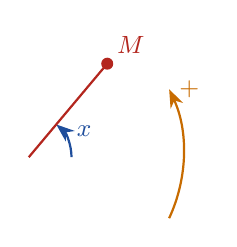
\begin{tikzpicture}[scale=1.55,font=\small]
\TrigCircle
\draw[cDef,thick,-{Stealth}] (0.35,0) arc(0:50:0.35);
\draw[cThm,thick] (0,0)--(50:1);
\fill[cThm] (50:1) circle(1.4pt) node[above right]{$M$};
\node[cDef] at (25:0.5){$x$};
\draw[cEx,-{Stealth},thick] (1.15,-0.5) arc(-25:25:1.25) node[right]{$+$};
\end{tikzpicture}
\end{LTR}\end{center}}

% =====================================================================
\section{الزاوية الموجهة لشعاعين وأقياسها}
\begin{tarif}
$\vu$ و $\vv$ شعاعان غير معدومين. \ الثنائية $\an{\vu}{\vv}$ تسمى \textbf{زاوية موجهة} للشعاعين $\vu$ و $\vv$.\par
نرسم $\V{OM}=\dfrac{\vu}{\|\vu\|}$ و $\V{ON}=\dfrac{\vv}{\|\vv\|}$ حيث $M$ و $N$ على الدائرة المثلثية. \ إذا كان $x$ قيساً للقوس الموجه من $M$ إلى $N$ فإن:
\begin{itemize}
\item $x$ هو \textbf{قيس} للزاوية الموجهة $\an{\vu}{\vv}$ بالراديان.
\item كل الأعداد \bx{x+2k\pi} ($k\in\Z$) هي أيضاً أقياس لنفس الزاوية ، ونكتب تجاوزاً: $\an{\vu}{\vv}=x+2k\pi$ أو $\an{\vu}{\vv}=x$.
\end{itemize}
\end{tarif}
\begin{khassia}[قيسان لنفس الزاوية]
العددان $\alpha$ و $\alpha'$ قيسان لنفس الزاوية الموجهة \ $\iff$ \ \bx{\alpha'-\alpha=2k\pi} مع $k\in\Z$ \ (أي فرقهما مضاعف للعدد $2\pi$).
\end{khassia}
\begin{mithal}
\begin{itemize}
\item هل $\dfrac{11\pi}{4}$ و $-\dfrac{5\pi}{4}$ قيسان لنفس الزاوية؟ \ $\dfrac{11\pi}{4}-\Big(-\dfrac{5\pi}{4}\Big)=\dfrac{16\pi}{4}=4\pi=2\times2\pi$: \textbf{نعم}.
\item هل $\dfrac{11\pi}{2}$ و $\dfrac{9\pi}{2}$ قيسان لنفس الزاوية؟ \ $\dfrac{11\pi}{2}-\dfrac{9\pi}{2}=\pi$ وليس مضاعفاً لـ $2\pi$: \textbf{لا}.
\end{itemize}
\end{mithal}

% =====================================================================
\section{القيس الرئيسي}
\begin{khassia}[تعريف وخاصية]
من بين أقياس الزاوية الموجهة $\an{\vu}{\vv}$ يوجد قيس \textbf{وحيد} ينتمي إلى المجال \bx{]-\pi;\pi]} ، يسمى \textbf{القيس الرئيسي}.\par
إذا كان $\alpha$ القيس الرئيسي لـ $\an{\vu}{\vv}$ فإن $|\alpha|$ هو قيس الزاوية الهندسية (غير الموجهة) المكونة من $\vu$ و $\vv$.
\end{khassia}
\begin{molahada}[قيم خاصة]
\begin{center}
\renewcommand{\arraystretch}{1.5}
\begin{tabular}{|c|c|c|c|C|}\hline
\ar{قائمة غير مباشرة} & \ar{قائمة مباشرة} & $\an{\vu}{-\vu}$ & $\an{\vu}{\vu}$ & الزاوية\\\hline
$-\dfrac{\pi}{2}$ & $\dfrac{\pi}{2}$ & $\pi$ & $0$ & القيس الرئيسي\\\hline
\end{tabular}
\end{center}
\end{molahada}
\begin{tariqa}[تعيين القيس الرئيسي لزاوية قيسها $\alpha=\dfrac{p\pi}{q}$]
\textbf{الطريقة 1 (الحصر):} نبحث عن العدد الصحيح $k$ حيث \bx{-\pi<\alpha+2k\pi\le\pi} ، فيكون القيس الرئيسي $\alpha+2k\pi$.\par
\textbf{الطريقة 2 (القسمة):} نكتب $p=2q\cdot n+r$ لنحصل على $\alpha=2n\pi+\dfrac{r\pi}{q}$ مع $\dfrac{r\pi}{q}\in\,]-\pi;\pi]$.
\end{tariqa}
\begin{mithal}
\textbf{1.} $\alpha=\dfrac{65\pi}{3}$. \ \textbf{بالحصر:} $-\pi<\dfrac{65\pi}{3}+2k\pi\le\pi\iff-1<\dfrac{65}{3}+2k\le1\iff-\dfrac{68}{6}<k\le-\dfrac{62}{6}$ ، أي $-11{,}33<k\le-10{,}33$ ، ومنه $k=-11$:
\[\dfrac{65\pi}{3}-22\pi=\dfrac{65\pi-66\pi}{3}=\bx{-\dfrac{\pi}{3}}.\]
\textbf{2.} $\alpha=-\dfrac{189\pi}{4}=-\dfrac{192\pi-3\pi}{4}=-48\pi+\dfrac{3\pi}{4}=-24(2\pi)+\dfrac{3\pi}{4}$: \ القيس الرئيسي \bx{\dfrac{3\pi}{4}}.\par
\textbf{3.} $\alpha=\dfrac{2025\pi}{4}=\dfrac{2024\pi+\pi}{4}=506\pi+\dfrac{\pi}{4}=253(2\pi)+\dfrac{\pi}{4}$: \ القيس الرئيسي \bx{\dfrac{\pi}{4}}.\par
\textbf{4.} $\alpha=-\dfrac{35\pi}{2}=\dfrac{-36\pi+\pi}{2}=-18\pi+\dfrac{\pi}{2}$: \ القيس الرئيسي \bx{\dfrac{\pi}{2}}.
\end{mithal}

% =====================================================================
\section{خواص الزوايا الموجهة}
\begin{khassia}[علاقة شال]
من أجل كل ثلاثة أشعة غير معدومة $\vu$ ، $\vv$ و $\vw$:
\[\bx{\an{\vu}{\vv}+\an{\vv}{\vw}=\an{\vu}{\vw}}\qquad(2\pi).\]
\end{khassia}
\begin{khassia}[نتائج]
من أجل كل شعاعين غير معدومين $\vu$ و $\vv$:
\begin{center}
\renewcommand{\arraystretch}{1.5}
\begin{tabular}{|c|c|c|c|}\hline
$\an{\vv}{\vu}=-\an{\vu}{\vv}$ & $\an{\vu}{-\vv}=\an{\vu}{\vv}+\pi$ & $\an{-\vu}{\vv}=\an{\vu}{\vv}+\pi$ & $\an{-\vu}{-\vv}=\an{\vu}{\vv}$\\\hline
\end{tabular}
\end{center}
\end{khassia}
\begin{khassia}[ضرب شعاعين في عددين]
$k$ و $k'$ عددان حقيقيان غير معدومين:
\begin{itemize}
\item إذا كان $k$ و $k'$ \textbf{من نفس الإشارة}: \ \bx{\an{k\vu}{k'\vv}=\an{\vu}{\vv}}.
\item إذا كان $k$ و $k'$ \textbf{مختلفين في الإشارة}: \ \bx{\an{k\vu}{k'\vv}=\an{\vu}{\vv}+\pi}.
\end{itemize}
\end{khassia}
\begin{khassia}[الزاوية الموجهة والارتباط الخطي]
$\vu$ و $\vv$ مرتبطان خطياً \ $\iff$ \ $\an{\vu}{\vv}=0+2k\pi$ (نفس الاتجاه) \ أو \ $\an{\vu}{\vv}=\pi+2k\pi$ (اتجاهان متعاكسان).\par
\textbf{تطبيقات:} \ $A$ ، $B$ ، $C$ على استقامة واحدة $\iff\an{\V{AB}}{\V{AC}}=k\pi$ \ ؛ \ $(AB)\parallel(CD)\iff\an{\V{AB}}{\V{CD}}=k\pi$.\par
\textbf{التعامد:} $(AB)\perp(CD)\iff\an{\V{AB}}{\V{CD}}=\dfrac{\pi}{2}+k\pi$.
\end{khassia}
\begin{mithal}
علماً أن $\an{\vu}{\vv}=-\dfrac{\pi}{3}$:
\begin{itemize}
\item $\an{\vv}{\vu}=\dfrac{\pi}{3}$ \ ؛ \ $\an{-\vu}{-\vv}=-\dfrac{\pi}{3}$ \ ؛ \ $\an{-\vu}{\vv}=-\dfrac{\pi}{3}+\pi=\dfrac{2\pi}{3}$.
\item $\an{2\vv}{-\vu}$: $2$ و $-1$ مختلفان في الإشارة: $\an{\vv}{\vu}+\pi=\dfrac{\pi}{3}+\pi=\dfrac{4\pi}{3}$ ، والقيس الرئيسي \bx{-\dfrac{2\pi}{3}}.
\end{itemize}
\end{mithal}

\begin{tmr}
$ABC$ مثلث متقايس الأضلاع مباشر (أي $\an{\V{AB}}{\V{AC}}=\dfrac{\pi}{3}$). \ عيّن القيس الرئيسي لكل من الزوايا:
\[\an{\V{AB}}{\V{BC}}\qquad;\qquad\an{\V{CA}}{\V{CB}}\qquad;\qquad\an{\V{BA}}{-2\V{CA}}\qquad;\qquad\an{\V{CB}}{3\V{AB}}.\]
\end{tmr}
\begin{hal}
في المثلث المتقايس الأضلاع المباشر: $\an{\V{AB}}{\V{AC}}=\an{\V{BC}}{\V{BA}}=\an{\V{CA}}{\V{CB}}=\dfrac{\pi}{3}$.
\begin{itemize}
\item $\an{\V{AB}}{\V{BC}}=\an{-\V{BA}}{\V{BC}}=\an{\V{BA}}{\V{BC}}+\pi=-\dfrac{\pi}{3}+\pi=\bx{\dfrac{2\pi}{3}}$.
\item $\an{\V{CA}}{\V{CB}}=\bx{\dfrac{\pi}{3}}$.
\item $\an{\V{BA}}{-2\V{CA}}=\an{\V{BA}}{\V{CA}}+\pi$. \ و $\an{\V{BA}}{\V{CA}}=\an{\V{AB}}{\V{AC}}=\dfrac{\pi}{3}$ (لأن $\an{-\vu}{-\vv}=\an{\vu}{\vv}$) ، إذن: $\dfrac{\pi}{3}+\pi=\dfrac{4\pi}{3}$ ، والقيس الرئيسي \bx{-\dfrac{2\pi}{3}}.
\item $\an{\V{CB}}{3\V{AB}}=\an{\V{CB}}{\V{AB}}$ \ ($1$ و $3$ موجبان). \ ولدينا $\an{\V{BC}}{\V{BA}}=\dfrac{\pi}{3}$ ، و $\an{\V{CB}}{\V{AB}}=\an{-\V{BC}}{-\V{BA}}=\an{\V{BC}}{\V{BA}}=\bx{\dfrac{\pi}{3}}$.
\end{itemize}
\end{hal}

% =====================================================================
\section{الزاوية المحيطية والزاوية المركزية}
\RL{0.56}{%
\begin{khassia}[مبرهنة الزاوية المحيطية]
$(C)$ دائرة مركزها $O$ ، و $A$ ، $B$ ، $M$ ثلاث نقط متمايزة منها.\par
إذا كان $\alpha$ قيساً للزاوية المركزية $\an{\V{OA}}{\V{OB}}$ فإن \bx{\dfrac{\alpha}{2}} قيس للزاوية المحيطية $\an{\V{MA}}{\V{MB}}$ ، أي:
\[\bx{2\an{\V{MA}}{\V{MB}}=\an{\V{OA}}{\V{OB}}}\qquad(2\pi).\]
\end{khassia}
\textbf{فكرة البرهان:} المثلثان $OAM$ و $OBM$ متساويا الساقين ، نستعمل علاقة شال ومجموع زوايا المثلث.}
{0.4}{%
\begin{center}\begin{LTR}
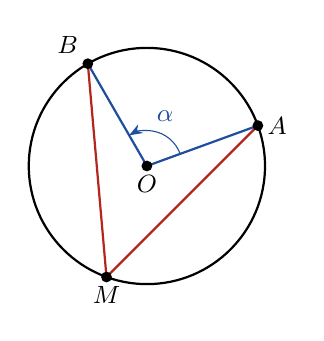
\begin{tikzpicture}[scale=1.5,font=\small]
\draw[thick] (0,0) circle(1);
\coordinate (O) at (0,0); \coordinate (A) at (20:1); \coordinate (B) at (120:1); \coordinate (M) at (250:1);
\draw[cDef,thick] (O)--(A); \draw[cDef,thick] (O)--(B);
\draw[cThm,thick] (M)--(A); \draw[cThm,thick] (M)--(B);
\fill (O) circle(1.3pt) node[below]{$O$};
\fill (A) circle(1.3pt) node[right]{$A$}; \fill (B) circle(1.3pt) node[above left]{$B$};
\fill (M) circle(1.3pt) node[below]{$M$};
\draw[cDef,-{Stealth}] (20:0.3) arc(20:120:0.3); \node[cDef] at (70:0.45){$\alpha$};
\end{tikzpicture}
\end{LTR}\end{center}}

% =====================================================================
\section{جيب التمام والجيب: القيم الشهيرة}
\RL{0.55}{%
\begin{tarif}
$M$ صورة العدد الحقيقي $x$ على الدائرة المثلثية في المعلم المتعامد والمتجانس المباشر $(O;\vec i,\vec j)$:
\begin{itemize}
\item \textbf{جيب تمام} $x$ ($\cos x$) هو فاصلة $M$ ، و\textbf{جيب} $x$ ($\sin x$) هو ترتيب $M$.
\end{itemize}
\end{tarif}
\begin{khassia}[خواص]
من أجل كل عدد حقيقي $x$ ومن أجل كل $k\in\Z$:
\begin{itemize}
\item $-1\le\cos x\le1$ \ و \ $-1\le\sin x\le1$ \ ؛ \ \bx{\cos^2x+\sin^2x=1}.
\item $\cos(x+2k\pi)=\cos x$ \ و \ $\sin(x+2k\pi)=\sin x$ (دوريتان ودورهما $2\pi$).
\end{itemize}
\end{khassia}}
{0.42}{%
\begin{center}\begin{LTR}
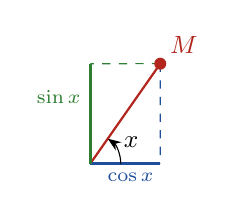
\begin{tikzpicture}[scale=1.55,font=\small]
\TrigCircle
\coordinate (M) at (55:1);
\draw[cThm,thick] (0,0)--(M);
\draw[cDef,dashed] (M)--(0.5736,0); \draw[cRem,dashed] (M)--(0,0.8192);
\draw[cDef,very thick] (0,0)--(0.5736,0); \draw[cRem,very thick] (0,0)--(0,0.8192);
\fill[cThm] (M) circle(1.4pt) node[above right]{$M$};
\node[cDef,below,font=\scriptsize] at (0.33,0){$\cos x$};
\node[cRem,left,font=\scriptsize] at (0,0.55){$\sin x$};
\draw[-{Stealth}] (0.25,0) arc(0:55:0.25); \node at (28:0.38){$x$};
\end{tikzpicture}
\end{LTR}\end{center}}
\begin{khassia}[جدول القيم الشهيرة]
\begin{center}
\renewcommand{\arraystretch}{1.8}
\begin{tabular}{|c|c|c|c|c|c|c|}\hline
$x$ & $0$ & $\dfrac{\pi}{6}$ & $\dfrac{\pi}{4}$ & $\dfrac{\pi}{3}$ & $\dfrac{\pi}{2}$ & $\pi$\\\hline
$\cos x$ & $1$ & $\dfrac{\sqrt3}{2}$ & $\dfrac{\sqrt2}{2}$ & $\dfrac12$ & $0$ & $-1$\\\hline
$\sin x$ & $0$ & $\dfrac12$ & $\dfrac{\sqrt2}{2}$ & $\dfrac{\sqrt3}{2}$ & $1$ & $0$\\\hline
\end{tabular}
\end{center}
\end{khassia}

% =====================================================================
\section{الزوايا المرفقة (دساتير التحويل)}
\begin{khassia}
من أجل كل عدد حقيقي $x$:
\begin{center}
\renewcommand{\arraystretch}{1.8}
\begin{tabular}{|C|c|c|C|}\hline
التفسير الهندسي (الصورتان $M$ و $M'$) & $\sin$ & $\cos$ & الزاوية\\\hline
متناظرتان بالنسبة لمحور الفواصل & $\sin(-x)=-\sin x$ & $\cos(-x)=\cos x$ & $-x$\\\hline
متناظرتان بالنسبة لمحور التراتيب & $\sin(\pi-x)=\sin x$ & $\cos(\pi-x)=-\cos x$ & $\pi-x$\\\hline
متناظرتان بالنسبة للمبدأ $O$ & $\sin(\pi+x)=-\sin x$ & $\cos(\pi+x)=-\cos x$ & $\pi+x$\\\hline
متناظرتان بالنسبة للمستقيم $y=x$ & $\sin\big(\frac{\pi}{2}-x\big)=\cos x$ & $\cos\big(\frac{\pi}{2}-x\big)=\sin x$ & $\dfrac{\pi}{2}-x$\\\hline
دوران بربع دورة & $\sin\big(\frac{\pi}{2}+x\big)=\cos x$ & $\cos\big(\frac{\pi}{2}+x\big)=-\sin x$ & $\dfrac{\pi}{2}+x$\\\hline
\end{tabular}
\end{center}
\end{khassia}
\begin{center}\begin{LTR}
\begin{tikzpicture}[scale=1.25,font=\scriptsize]
\begin{scope}
\TrigCircle
\draw[cThm,thick] (0,0)--(35:1); \fill[cThm] (35:1) circle(1.3pt) node[right]{$M(x)$};
\draw[cDef,thick] (0,0)--(-35:1); \fill[cDef] (-35:1) circle(1.3pt) node[right]{$-x$};
\draw[dashed] (35:1)--(-35:1);
\end{scope}
\begin{scope}[xshift=3.3cm]
\TrigCircle
\draw[cThm,thick] (0,0)--(35:1); \fill[cThm] (35:1) circle(1.3pt) node[right]{$x$};
\draw[cDef,thick] (0,0)--(145:1); \fill[cDef] (145:1) circle(1.3pt) node[left]{$\pi-x$};
\draw[dashed] (35:1)--(145:1);
\end{scope}
\begin{scope}[xshift=6.6cm]
\TrigCircle
\draw[cThm,thick] (0,0)--(35:1); \fill[cThm] (35:1) circle(1.3pt) node[right]{$x$};
\draw[cDef,thick] (0,0)--(215:1); \fill[cDef] (215:1) circle(1.3pt) node[left]{$\pi+x$};
\end{scope}
\begin{scope}[xshift=9.9cm]
\TrigCircle
\draw[gray,dashed] (-1.1,-1.1)--(1.15,1.15);
\draw[cThm,thick] (0,0)--(25:1); \fill[cThm] (25:1) circle(1.3pt) node[right]{$x$};
\draw[cDef,thick] (0,0)--(65:1); \fill[cDef] (65:1) circle(1.3pt) node[above]{$\frac{\pi}{2}-x$};
\end{scope}
\end{tikzpicture}
\end{LTR}\end{center}

\begin{tariqa}[حساب جيب أو جيب تمام عدد كبير]
نكتب العدد على الشكل $x_0+2k\pi$ (نحذف الدورات الكاملة) ، ثم نستعمل الزوايا المرفقة للرجوع إلى زاوية شهيرة.
\end{tariqa}
\begin{mithal}
\begin{itemize}
\item $\sin\dfrac{193\pi}{3}=\sin\Big(64\pi+\dfrac{\pi}{3}\Big)=\sin\dfrac{\pi}{3}=\bx{\dfrac{\sqrt3}{2}}$.
\item $\cos\dfrac{17\pi}{6}=\cos\Big(2\pi+\dfrac{5\pi}{6}\Big)=\cos\Big(\pi-\dfrac{\pi}{6}\Big)=-\cos\dfrac{\pi}{6}=\bx{-\dfrac{\sqrt3}{2}}$.
\item $\sin\dfrac{55\pi}{4}=\sin\Big(14\pi-\dfrac{\pi}{4}\Big)=\sin\Big(-\dfrac{\pi}{4}\Big)=\bx{-\dfrac{\sqrt2}{2}}$.
\item $\cos\dfrac{4\pi}{3}=\cos\Big(\pi+\dfrac{\pi}{3}\Big)=-\cos\dfrac{\pi}{3}=\bx{-\dfrac12}$ \ ؛ \ $\sin\dfrac{2\pi}{3}=\sin\Big(\pi-\dfrac{\pi}{3}\Big)=\bx{\dfrac{\sqrt3}{2}}$.
\end{itemize}
\end{mithal}
\begin{mithal}[تبسيط عبارة]
$A=\sin(x+5\pi)+\sin\Big(\dfrac{3\pi}{2}-x\Big)+\cos\Big(\dfrac{\pi}{2}-x\Big)$.
\begin{itemize}
\item $\sin(x+5\pi)=\sin(x+\pi+4\pi)=\sin(\pi+x)=-\sin x$.
\item $\sin\Big(\dfrac{3\pi}{2}-x\Big)=\sin\Big(2\pi-\dfrac{\pi}{2}-x\Big)=\sin\Big(-\big(\tfrac{\pi}{2}+x\big)\Big)=-\sin\Big(\dfrac{\pi}{2}+x\Big)=-\cos x$.
\item $\cos\Big(\dfrac{\pi}{2}-x\Big)=\sin x$.
\end{itemize}
إذن: $A=-\sin x-\cos x+\sin x=\bx{-\cos x}$.
\end{mithal}

% =====================================================================
\section{المعادلات المثلثية الأساسية}
\begin{khassia}[الأعداد التي لها نفس جيب التمام أو نفس الجيب]
$a$ و $b$ عددان حقيقيان ، $k\in\Z$:
\[\bx{\cos a=\cos b\iff a=b+2k\pi\ \ \text{\ar{أو}}\ \ a=-b+2k\pi}\]
\[\bx{\sin a=\sin b\iff a=b+2k\pi\ \ \text{\ar{أو}}\ \ a=\pi-b+2k\pi}\]
\end{khassia}
\begin{tariqa}[حل المعادلة $\cos x=a$ (أو $\sin x=a$)]
\begin{enumerate}
\item إذا كان $a\notin[-1;1]$: المعادلة \textbf{لا تقبل حلولاً} في $\R$.
\item إذا كان $a\in[-1;1]$: نبحث عن عدد شهير $b$ حيث $\cos b=a$ (أو $\sin b=a$) ، ثم نطبق الخاصية السابقة.
\item لتعيين الحلول في مجال $I$: نعوّض $k$ بقيم صحيحة ونحتفظ بالحلول التي تنتمي إلى $I$ (أو نحصر $k$).
\end{enumerate}
\textbf{حالات خاصة:} $\cos x=0\iff x=\dfrac{\pi}{2}+k\pi$ \ ؛ \ $\sin x=0\iff x=k\pi$ \ ؛ \ $\cos x=1\iff x=2k\pi$ \ ؛ \ $\sin x=1\iff x=\dfrac{\pi}{2}+2k\pi$.
\end{tariqa}
\begin{mithal}
\textbf{1.} $\cos x=\dfrac{\sqrt3}{2}=\cos\dfrac{\pi}{6}$: \ $S=\Big\{\dfrac{\pi}{6}+2k\pi\,;\,-\dfrac{\pi}{6}+2k\pi\,/\,k\in\Z\Big\}$.\par
\textbf{2.} $\cos x=-\dfrac{\sqrt2}{2}=\cos\dfrac{3\pi}{4}$: \ $S=\Big\{\dfrac{3\pi}{4}+2k\pi\,;\,-\dfrac{3\pi}{4}+2k\pi\,/\,k\in\Z\Big\}$.\par
\textbf{3.} $\sin x=\dfrac{\sqrt2}{2}=\sin\dfrac{\pi}{4}$: \ $x=\dfrac{\pi}{4}+2k\pi$ أو $x=\pi-\dfrac{\pi}{4}+2k\pi=\dfrac{3\pi}{4}+2k\pi$.\par
\textbf{4.} $\sin x=-\dfrac12=\sin\Big(-\dfrac{\pi}{6}\Big)$: \ $x=-\dfrac{\pi}{6}+2k\pi$ أو $x=\dfrac{7\pi}{6}+2k\pi$.\par
\textbf{5. في مجال:} $\cos x=\dfrac12$ في $[-\pi;3\pi]$: الحلول $\dfrac{\pi}{3}+2k\pi$ و $-\dfrac{\pi}{3}+2k\pi$:
\begin{itemize}
\item $\dfrac{\pi}{3}+2k\pi$: $k=0\to\dfrac{\pi}{3}$ ، $k=1\to\dfrac{7\pi}{3}$ مقبولان ، $k=2\to\dfrac{13\pi}{3}$ مرفوض.
\item $-\dfrac{\pi}{3}+2k\pi$: $k=0\to-\dfrac{\pi}{3}$ ، $k=1\to\dfrac{5\pi}{3}$ مقبولان ، $k=-1\to-\dfrac{7\pi}{3}$ مرفوض.
\end{itemize}
$S=\Big\{-\dfrac{\pi}{3};\dfrac{\pi}{3};\dfrac{5\pi}{3};\dfrac{7\pi}{3}\Big\}$.
\end{mithal}
\begin{tariqa}[معادلة من الشكل $\cos u=\sin v$]
نحوّل $\sin$ إلى $\cos$ باستعمال $\sin v=\cos\Big(\dfrac{\pi}{2}-v\Big)$ ، ثم نحل $\cos u=\cos\Big(\dfrac{\pi}{2}-v\Big)$.\par
\textbf{مثال:} $\cos2x=\sin x\iff\cos2x=\cos\Big(\dfrac{\pi}{2}-x\Big)$:
\begin{itemize}
\item $2x=\dfrac{\pi}{2}-x+2k\pi\iff x=\dfrac{\pi}{6}+\dfrac{2k\pi}{3}$ \ ؛ \ أو \ $2x=-\dfrac{\pi}{2}+x+2k\pi\iff x=-\dfrac{\pi}{2}+2k\pi$.
\end{itemize}
\end{tariqa}

% =====================================================================
\section{المتراجحات المثلثية}
\begin{tariqa}[حل متراجحة مثلثية في مجال باستعمال الدائرة المثلثية]
\begin{enumerate}
\item نحل المعادلة المرفقة في المجال المطلوب (نقط الحدود $M_1$ ، $M_2$).
\item نمثل على الدائرة المثلثية: لـ $\cos x\le a$ نرسم المستقيم العمودي $x=a$ ، ولـ $\sin x\le a$ نرسم المستقيم الأفقي $y=a$.
\item نعيّن القوس الذي تحقق نقطه المتراجحة ، ثم نكتب الحلول كاتحاد مجالات من المجال المطلوب.
\end{enumerate}
\end{tariqa}
\RL{0.55}{%
\begin{mithal}
حل في $[0;2\pi[$ المتراجحة $\sin x<\dfrac12$.\par
$\sin x=\dfrac12$ في $[0;2\pi[$: $x=\dfrac{\pi}{6}$ أو $x=\dfrac{5\pi}{6}$.\par
تكون $\sin x<\dfrac12$ عندما تكون $M$ \textbf{تحت} المستقيم $y=\dfrac12$ (القوس الأحمر):
\[\bx{S=\Big[0;\frac{\pi}{6}\Big[\,\cup\,\Big]\frac{5\pi}{6};2\pi\Big[}.\]
\end{mithal}}
{0.4}{%
\begin{center}\begin{LTR}
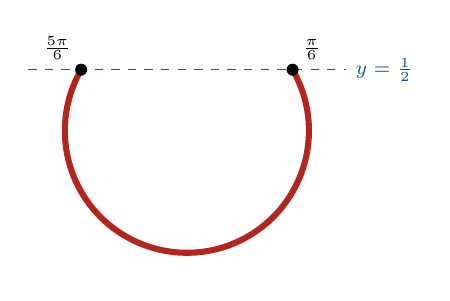
\begin{tikzpicture}[scale=1.55,font=\scriptsize]
\TrigCircle
\draw[cDef,dashed] (-1.3,0.5)--(1.3,0.5) node[right]{$y=\frac12$};
\draw[cThm,line width=2.2pt] (30:1) arc(30:-210:1);
\fill (30:1) circle(1.4pt) node[above right]{$\frac{\pi}{6}$};
\fill (150:1) circle(1.4pt) node[above left]{$\frac{5\pi}{6}$};
\end{tikzpicture}
\end{LTR}\end{center}}
\RL{0.55}{%
\begin{mithal}
حل في $]-\pi;\pi]$ المتراجحة $\sqrt2\cos x-1\le0$ ، أي $\cos x\le\dfrac{\sqrt2}{2}$.\par
$\cos x=\dfrac{\sqrt2}{2}$ في $]-\pi;\pi]$: $x=\pm\dfrac{\pi}{4}$.\par
تكون $\cos x\le\dfrac{\sqrt2}{2}$ عندما تكون $M$ \textbf{على يسار} المستقيم $x=\dfrac{\sqrt2}{2}$:
\[\bx{S=\Big]-\pi;-\frac{\pi}{4}\Big]\,\cup\,\Big[\frac{\pi}{4};\pi\Big]}.\]
\end{mithal}}
{0.4}{%
\begin{center}\begin{LTR}
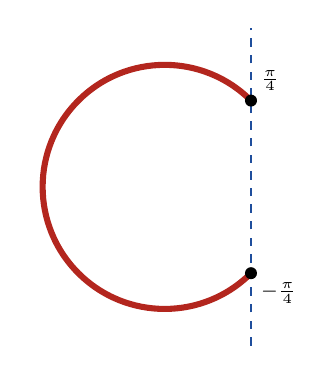
\begin{tikzpicture}[scale=1.55,font=\scriptsize]
\TrigCircle
\draw[cDef,dashed] (0.7071,-1.3)--(0.7071,1.3);
\draw[cThm,line width=2.2pt] (45:1) arc(45:315:1);
\fill (45:1) circle(1.4pt) node[above right]{$\frac{\pi}{4}$};
\fill (-45:1) circle(1.4pt) node[below right]{$-\frac{\pi}{4}$};
\end{tikzpicture}
\end{LTR}\end{center}}

% =====================================================================
\section{خلاصة الطرائق}
\begin{BOX}{cMeth}{ماذا أفعل عندما يُطلب مني $\ldots$؟}
\renewcommand{\arraystretch}{1.5}
\centering
\begin{tabular}{|p{0.52\textwidth}|p{0.36\textwidth}|}\hline
\cellcolor{cMeth!15}\textbf{الطريقة} & \cellcolor{cMeth!15}\textbf{المطلوب}\\\hline
نحسب الفرق: إذا كان مضاعفاً لـ $2\pi$ فهما قيسان لنفس الزاوية. & هل $\alpha$ و $\alpha'$ قيسان لنفس الزاوية؟\\\hline
نحصر $-\pi<\alpha+2k\pi\le\pi$ ، أو نحذف الدورات الكاملة. & القيس الرئيسي\\\hline
علاقة شال ، $\an{-\vu}{\vv}=\an{\vu}{\vv}+\pi$ ، إشارتا $k$ و $k'$. & قيس زاوية بدلالة زاوية معلومة\\\hline
$\an{\V{AB}}{\V{AC}}=k\pi$. & استقامية / توازي\\\hline
$2\an{\V{MA}}{\V{MB}}=\an{\V{OA}}{\V{OB}}$. & زاوية محيطية\\\hline
حذف الدورات ثم الزوايا المرفقة. & $\cos$ أو $\sin$ لعدد كبير\\\hline
$\cos a=\cos b$ أو $\sin a=\sin b$ ، ثم تحويل $\sin$ إلى $\cos$ عند الحاجة. & معادلة مثلثية\\\hline
الحلول الحدية ثم القوس المناسب على الدائرة المثلثية. & متراجحة مثلثية\\\hline
\end{tabular}
\end{BOX}

\end{document}
